\documentclass{beamer}

%\usepackage{beamerthemesplit}
\usepackage{pgfpages,threeparttable,graphics,amsmath,amssymb,overpic}
%\setbeameroption{previous slide on second screen}
%\pgfpagesuselayout{4 on 1}[a4paper,border shrink=5mm,landscape]
\newtheorem{assump}{Assumption}
\newtheorem{imp}{Implication}[assump]
\newtheorem{hypo}{Hypothesis}
\newtheorem{prop}{Proposition}
\newtheorem{impl}{Implication}[prop]
\newtheorem{genhyp}{General Hypothesis}
\newtheorem{defi}{Definition}
\newcounter{saveenumi}
\title[Nothing at All]{Is Doing Nothing Something? }
\author{Me \and Myself \and I}

%\date{January  2016}
 
 
\mode<presentation>
{
  \usetheme{AnnArbor}
\usecolortheme{beaver}
  \setbeamercovered{transparent}
}
%there are lots of themes - see http://deic.uab.es/~iblanes/beamer_gallery/index_by_theme.html
  % you can alter them and create your own pretty easily.
  
%some options below
%\pgfdeclareimage[height=0.5cm]{BUlogo}{bulogonew}
%\logo{\pgfuseimage{BUlogo}}

% \setbeamercolor{block body example}{fg=blue,bg=white}
 %\setbeamercolor{block title example}{fg=blue,bg=lightgray}
 
\begin{document}
% \begin{frame} {slide title} \end{frame}
\frame{\titlepage}

\frame{{Relaxing Assumptions about doing something and nothing}

\begin{itemize}
\item the first thing \pause
\item the second thing \pause
\item the third thing \pause
\end{itemize}

It is improbable doing nothing is the same as not doing something, yet strong evidence of this exists.
}

\frame{{The Problem with Something}
These reasonable claims obscure two things: 

\begin{enumerate} \pause
\item thing 1 \pause
\item thing 2 
\end{enumerate} 



}


\frame{{Theory of Nothing}
 
Our strategy is to examine how doing nothing amounts to doing something because: 

\begin{itemize} \pause
\item reason 1 \pause
\item reason b \pause
\end{itemize} ~\\

and measure the differences in these effects before and after doing nothing. 
}
 
  
\frame{{Some Results}
\begin{tiny}

\begin{table}[ht]
\begin{center}
\begin{threeparttable}
\caption{Something or Nothing?\tnote{\dag}} \label{tab:somenumbers}
\begin{tabular}{lrrr}
\hline \hline
 &Coefficient  &Std. Err. & z-score\\ \hline


Meaningful Variable 1	&	0.001	&	0.019	&	0.06	\\
Meaningful Variable 2	&	11.525	&	3.010	&	3.83	\\
Meaningful Variable 3 &	-1.296	&	0.529	&	-2.45	\\
intercept	&	-2.023	&	0.143	&	-14.16	\\ \\

N &a billion \\
model $\chi^2$	& 63.53*				\\ \hline

\hline \hline

\end{tabular}
\begin{tablenotes}
\item[\dag] {{ I made these up. You should not do this in a paper. * p $\leq$ .01}}
\end{tablenotes}
\end{threeparttable}
\end{center}
\end{table}
\end{tiny}

}


\frame{{Nothing and Something}

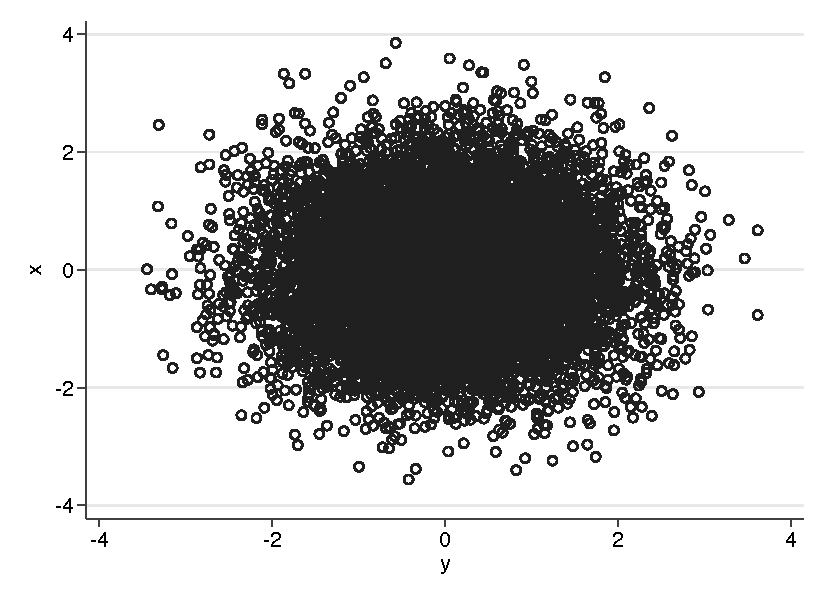
\includegraphics[width=4in]{somenumbers.pdf} 




}



\frame{{Conclusions}
Doing nothing is not always not the same as doing something.
\begin{itemize}
\item finding 1
\item finding 2
\item finding 3
\end{itemize}
}


\end{document}
 